%Câu 8
\begin{ex}%[2H3G1-4]
	Trong không gian với hệ trục tọa độ $Oxyz$, cho mặt cầu $(S) \colon (x-1)^2 + (y-2)^2 + (z+1)^2 = 9$ và hai điểm $A(4;3;1)$, $B(3;1;3)$; $M$ là điểm thay đổi trên $(S)$. Gọi $m,n$  lần lượt là giá trị lớn nhất và giá trị nhỏ nhất của biểu thức $P^2=2MA^2-MB^2$. Xác định $(m-n)$.
	\choice
	{$64$}
	{$68$}
	{\True $60$}
	{$48$}
	\loigiai{
		\begin{center}
			\begin{tikzpicture}
				\draw (2,0) circle(2cm);
				\filldraw (-2,0) circle(1.5pt) node[below] {I};
				\filldraw (0,0) circle(1.5pt) node[below left] {$M_1$};
				\filldraw (2,0) circle(1.5pt) node[below] {J};
				\filldraw (4,0) circle(1.5pt) node[below right] {$M_2$};
				\draw (-2,0) -- (4,0);
			\end{tikzpicture}
		\end{center}
		Gọi $I$ là điểm thỏa mãn $2\vec{IA}-\vec{IB}=\vec{0} \Rightarrow I(2x_A-x_B;2y_A-y_B;2z_A-z_B) \Rightarrow I(5;5;-1)$.\\
		Suy ra $I$ là điểm cố định. Vậy $P$ đạt giá trị nhỏ nhất khi $MI$ đạt giá trị nhỏ nhất, $P$ đạt giá trị lớn nhất khi $MI$ đạt giá trị lớn nhất.\\
		$\Rightarrow (S) \colon (x-1)^2 + (y-2)^2 + (z+1)^2 = 9$ có tâm $J(1;2;-1)$ và bán kính $R=3$.\\
		Ta có $IJ=5$ và $M$ là điểm thay đổi trên $(S)$. Do đó\\
		$\min MI=IM_1=IJ-R=5-3=2$ và $\max MI=IM_2=IJ+R=5+3=8$ $\Rightarrow m-n=8^2-2^2=60$.}
\end{ex}

%Câu 9
\begin{ex}%[2H3G1-4]
	Trong không gian với hệ trục tọa độ $Oxyz$, cho hai điểm $A(2;-2;4)$, $B(-3;3;-1)$ và mặt cầu $(S) \colon (x-1)^2+(y-3)^2+(z-3)^2=3$. Xét điểm $M$ thay đổi thuộc mặt cầu $(S)$, giá trị nhỏ nhất của $2MA^2+3MB^2$ bằng
	\choice
	{$103$}
	{$108$}
	{\True $105$}
	{$100$}
	\loigiai{
		\begin{center}
			\begin{tikzpicture}
				\draw (0,0) circle(2cm);
				\filldraw (0,0) circle(1.5pt) node[below left] {I};
				\filldraw (1.5,1.3) circle(1.5pt) node[right] {M};
				\filldraw (2.5,2.17) circle(1.5pt) node[above right] {E};
				\draw (0,0) -- (2.5,2.17);
			\end{tikzpicture}
		\end{center}
		Mặt cầu $(S)$ có tâm $I(1;3;3)$ bán kính $R=\sqrt3$.\\
		Gọi $E$ là điểm thỏa mãn: $2\vec{EA}+3\vec{EB}=\vec0$. Suy ra $E(-1;1;1)$.\\
		Xét $P=2MA^2+3MB^2=2(\vec{ME}+\vec{EA})^2+3(\vec{ME}+\vec{EB})^2=5ME^2+2EA^2+3EB^2$.\\
		$P$ đạt giá trị nhỏ nhất khi và chỉ khi $ME$ đạt giá trị nhỏ nhất và $IE=2\sqrt{3}>R$.\\ Suy ra điểm $E$ nằm ngoài mặt cầu nên $ME$ nhỏ nhất bằng\\
		$IE-R=2\sqrt{3}-\sqrt{3}=\sqrt{3}$.\\
		Vậy $P=2MA^2+3MB^2=5ME^2+2EA^2+3EB^2=105$.
	}
\end{ex}

%Câu 10
\begin{ex}%[2H3G1-4]
	Trong KG $Oxyz$, cho bốn điểm $A(1;0;0)$, $B(2;1;3)$, $C(0;2;-3)$, $D(2;0;\sqrt{7})$. Gọi $M$ là điểm thuộc mặt cầu $(S) \colon (x+2)^2+(y-4)^2+z^2=39$ thỏa mãn $MA^2+2\vec{MB}.\vec{MC}=8$. Biết rằng đoạn thẳng $MD$ đạt giá trị lớn nhất. Tìm giá trị lớn nhất đó.
	\choice
	{$\sqrt{7}$}
	{\True $2\sqrt{7}$}
	{$3\sqrt{7}$}
	{$4\sqrt{7}$}
	\loigiai{
		\begin{center}
			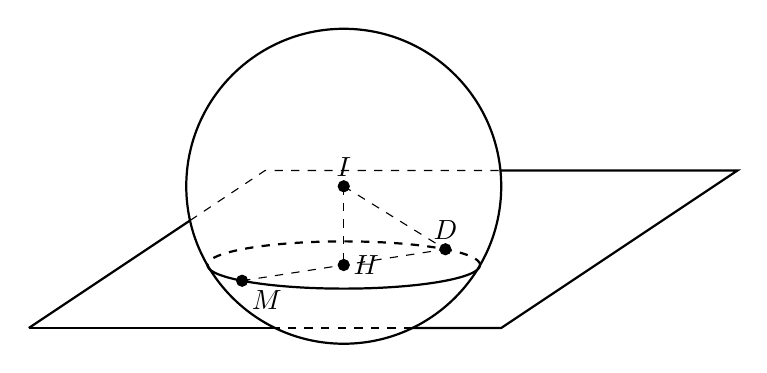
\begin{tikzpicture}
				\coordinate (P1) at (0,0);
				\coordinate (P2) at (2.04783,1.36522);
				\coordinate (P3) at (3,2);
				\coordinate (P4) at (5.989975,2);
				\coordinate (P5) at (9,2);
				\coordinate (P6) at (6,0);
				\coordinate (P7) at (4.871779,0);
				\coordinate (P8) at (3.12822,0);
				\coordinate (I) at (4,1.8);
				\coordinate (D) at (5.29099,1);
				\coordinate (H) at (4,0.8);
				\coordinate (M) at (2.709,0.6);
				\draw[thick] (P1) -- (P2);
				\draw[dashed] (P2) -- (P3) -- (P4);
				\draw[thick] (P4) -- (P5) -- (P6) -- (P7);
				\draw[dashed] (P7) -- (P8);
				\draw[thick] (P8) -- (P1);
				\draw[thick] (I) circle(2);
				\draw[dashed] (I) -- (H);
				\draw[dashed] (M) -- (D);
				\draw[dashed] (I) -- (D);
				\def\a{{sqrt(3)}}
				\def\b{0.3}
				\draw[dashed, thick] (5.732050807568878,0.8) arc[start angle=0, end angle=180, x radius=\a, y radius=\b];
				\draw[thick] (2.267949192431122,0.8) arc[start angle=180, end angle=360, x radius=\a, y radius=\b];
				\filldraw (I) circle(2pt) node[above] {$I$};
				\filldraw (D) circle(2pt) node[above] {$D$};
				\filldraw (H) circle(2pt) node[right] {$H$};
				\filldraw (M) circle(2pt) node[below right] {$M$};
			\end{tikzpicture}
		\end{center}
		Mặt cầu $(S) \colon (x+2)^2+(y-4)^2+z^2=39$ có tâm là $I(-2;4;0)$, bán kính $R=\sqrt{39}$.\\
		Gọi $M(x;y;z) \in (S)$. Ta có: $x^2+y^2+z^2=19-4x+8y$.\\
		$MA^2=(x-1)^2+y^2+z^2=20-6x+8y$.\\
		$\vec{MB}=(2-x;1-y;3-z)$; $\vec{MC}=(-x;2-y;-3-z)$.\\
		$\vec{MB} \cdot \vec{MC}=-2x+x^2+2-3y+y^2-9+z^2$$=19-4x+8y-2x-3y-7$ $=-6x+5y+12$.\\
		Suy ra $MA^2+2\vec{MB} \cdot \vec{MC}=-18x+18y+44$.\\
		Theo giả thiết $MA^2+2\vec{MB} \cdot \vec{MC}=8 \Leftrightarrow -18x+18y+44=8 \Leftrightarrow -x+y+2=0$.
		Do đó $M\in (P):-x+y+2=0$.\\
		Ta có $\mathrm{d}(I;(P))=\dfrac{\left| 8 \right|}{\sqrt{2}}=\sqrt{32}<\sqrt{39}$ nên mặt phẳng $(P)$ cắt mặt cầu $(S)$ theo giao tuyến là đường tròn $(C)$có bán kính $R_1$ với $R_1=\sqrt{R^2-d^2}=\sqrt{39-32}=\sqrt7$.\\
		Mặt khác ta có $\heva{&D,M \in (P)\\&D,M \in (S)} \Rightarrow D,M \in (C)$.\\
		Do đó độ dài $MD$ lớn nhất bằng $2R_1=2\sqrt{7}$.
	}
\end{ex}

%Câu 11
\begin{ex}%[2H3G1-4]
	Trong không gian tọa độ $Oxyz$, cho 5 điểm $A(1;0;0)$, $B(-1;1;0)$, $C(0;-1;0)$, $D(0;1;0)$, $E(0;3;0)$. $M$ là điểm thay đổi trên mặt cầu $(S) \colon x^2+(y-1)^2+z^2=1$. Giá trị lớn nhất của biểu thức $P=2\left| \vec{MA}+\vec{MB}+\vec{MC} \right|+3\left| \vec{MD}+\vec{ME} \right|$ là
	\choice
	{$12$}
	{\True $12\sqrt{2}$}
	{$24$}
	{$24\sqrt{2}$}
	\loigiai{
		Mặt cầu $(S)$ có tâm $I(0;1;0)$ bán kính $R=1$.\\
		Gọi trọng tâm tam giác $ABC$ là $G(0;0;0)$, trung điểm $DE$ là $N(0;2;0)$.\\
		do $G,N$ đều nằm trên $(S)$ và $I$ là trung điểm $GN$ nên $GN$ là đường kính của $(S)$.
		\begin{eqnarray*}
			&P&=2\left| \vec{MA}+\vec{MB}+\vec{MC} \right| +3\left|\vec{MD}+\vec{ME}\right|\\
			& &=2\left|3\vec{MG}\right| +3\left|\vec{MN}\right|\\
			& &=6MG+6MN=6(MG+MN)
		\end{eqnarray*}
		\begin{center}
			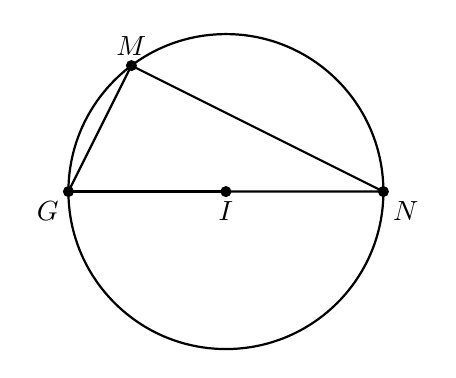
\begin{tikzpicture}
				\coordinate (G) at (-2, 0);
				\coordinate (I) at (0, 0);
				\coordinate (N) at (2, 0);
				\coordinate (M) at (-1.2, 1.6);
				\draw[thick] (I) circle (2);
				\draw[thick] (G) -- (M) -- (N) -- cycle;
				\draw[thick] (G) -- (I);
				\fill (G) circle (2pt);
				\fill (I) circle (2pt);
				\fill (N) circle (2pt);
				\fill (M) circle (2pt);
				\node[below left] at (G) {$G$};
				\node[below] at (I) {$I$};
				\node[below right] at (N) {$N$};
				\node[above] at (M) {$M$};
			\end{tikzpicture}
		\end{center}
		Ta có: $(MG+MN)^2\le 2(MG^2+MN^2)=2GN^2=8$.
		Suy ra $MG+MN\le 2\sqrt2$.\\
		Vậy giá trị lớn nhất của $P$ là $12\sqrt2$.
	}
\end{ex}

%Câu 12
\begin{ex}%[2H3G1-4]
	Trong không gian với hệ trục $Oxyz$, cho mặt cầu $(S) \colon (x+1)^2+(y-4)^2+z^2=8$ và điểm $A(3;0;0);B(4;2;1)$. Điểm $M$ thay đổi nằm trên mặt cầu, tìm giá trị nhỏ nhất của biểu thức $P=MA+2MB$.
	\choice
	{$P=2\sqrt{2}$}
	{$P=3\sqrt{2}$}
	{$P=4\sqrt{2}$}
	{\True $P=6\sqrt{2}$}
	\loigiai{
		\begin{center}
			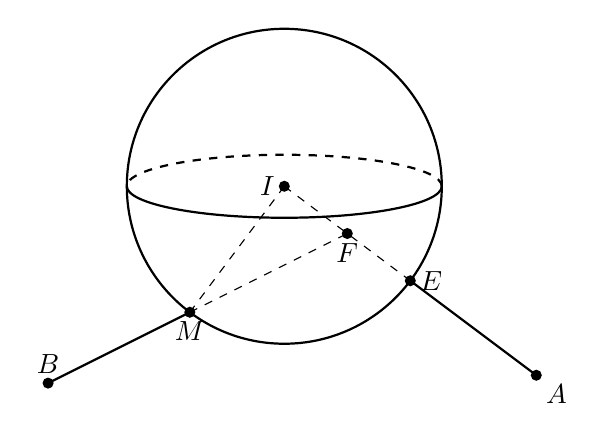
\begin{tikzpicture}
				\coordinate (E) at (1.6, -1.2);
				\coordinate (I) at (0, 0);
				\coordinate (A) at (3.2, -2.4);
				\coordinate (M) at (-1.2, -1.6);
				\coordinate (B) at (-3, -2.5);
				\coordinate (F) at (0.8, -0.6);
				\draw[thick] (I) circle (2);
				\draw[thick] (A) -- (E);
				\draw[dashed] (I) -- (E);
				\draw[thick] (M) -- (B);
				\draw[dashed] (M) -- (F);
				\draw[dashed] (I) -- (M);
				\def\a{2}
				\def\b{0.4}
				\draw[dashed, thick] (2,0) arc[start angle=0, end angle=180, x radius=\a, y radius=\b];
				\draw[thick] (-2,0) arc[start angle=180, end angle=360, x radius=\a, y radius=\b];
				\fill (E) circle (2pt);
				\fill (I) circle (2pt);
				\fill (A) circle (2pt);
				\fill (M) circle (2pt);
				\fill (B) circle (2pt);
				\fill (F) circle (2pt);
				\node[right] at (E) {$E$};
				\node[left] at (I) {$I$};
				\node[below right] at (A) {$A$};
				\node[below] at (M) {$M$};
				\node[above] at (B) {$B$};
				\node[below] at (F) {$F$};
			\end{tikzpicture}
		\end{center}
		Nhận xét: điểm $A,B$ nằm ngoài mặt cầu $(S)$. Mặt cầu $(S)$ có tâm $I(-1;4;0),R=2\sqrt2$.\\
		Ta có: $IA=4\sqrt2=2R,E=IA\cap (S)\Rightarrow E(1;2;0)$.\\
		Gọi $F$ là trung điểm của $IE\Rightarrow F(0;3;0)$.
		Tam giác $IFM$ và $IMA$ có $\widehat{AIM}$ chung và $\dfrac{IF}{IM}=\dfrac{1}{2}=\dfrac{IM}{IA} \Rightarrow \Delta AIM \sim \Delta MIF$.\\
		Suy ra $\dfrac{MA}{FM}=\dfrac{AI}{MI}=2\Rightarrow MA=2MF$.\\
		Ta có: $MA+2MB=2(MF+MB)\ge 2FB=6\sqrt2$.\\
		Vì $F$ nằm trong $(S)$ và $B$ nằm ngoài $(S)$ nên dấu $''=''$ xảy ra khi $M=BF \cap (S)$.\\
		Vậy giá trị nhỏ nhất là $P=6\sqrt{2}$.
	}
\end{ex}

%Câu 13 trùng 12
\begin{ex}%[2H3G1-4]
	Trong không gian với hệ trục $Oxyz$, cho mặt cầu $(S) \colon (x+1)^2+(y-4)^2+z^2=8$ và điểm $A(3;0;0)$, $B(4;2;1)$. Điểm $M$ thay đổi nằm trên mặt cầu, tìm giá trị nhỏ nhất của biểu thức $P=MA+2MB$.
	\choice
	{$P=2\sqrt{2}$}
	{$P=3\sqrt{2}$}
	{$P=4\sqrt{2}$}
	{\True $P=6\sqrt{2}$}
	\loigiai{
		Giả sử $M(x;y;z)$.
		Ta có: $\vec{AM}=(x-3;y;z)$, $\vec{BM}=(x-4;y-2;z-1)$.\\ Và $(x+1)^2+(y-4)^2+z^2=8$$\Leftrightarrow 3\left[ (x+1)^2+(y-4)^2+z^2-8 \right]=0$.\\
		Ta có:
		\begin{eqnarray*}
			&P&=MA+2MB\\
			&P&=\sqrt{(x-3)^2+y^2+z^2}+2\sqrt{(x-4)^2+(y-2)^2+(z-1)^2}\\
			&P&=\sqrt{(x-3)^2+y^2+z^2}+3\left[ (x+1)^2+(y-4)^2+z^2-8 \right]+2\sqrt{(x-4)^2+(y-2)^2+(z-1)^2}\\
			&P&=\sqrt{4x^2+4y^2-24y+4z^2+36}+2\sqrt{(x-4)^2+(y-2)^2+(z-1)^2}\\
			&P&=2\left[ \sqrt{x^2+(y-3)^2+z^2}+\sqrt{(x-4)^2+(y-2)^2+(z-1)^2} \right]\\
			&P&=2\left[ \sqrt{x^2+(y-3)^2+z^2}+\sqrt{(4-x)^2+(2-y)^2+(1-z)^2} \right]
		\end{eqnarray*}
		Áp dụng bất đẳng thức Minkowxki:\\
		$\sqrt{a^2+b^2+c^2}+\sqrt{d^2+e^2+f^2} \ge \sqrt{(a+d)^2+(b+e)^2+(c+f)^2}$.\\
		Dấu bằng xảy ra khi: $\dfrac{a}{d}=\dfrac{b}{e}=\dfrac{a}{f}>0$.\\
		$\Rightarrow P \ge 2\sqrt{(x+4-x)^2+(y-3+2-y)^2+(z+1-z)^2}=2\sqrt{4^2+(-1)^2+(1)^2}=6\sqrt{2}$.\\
		Dấu bằng xảy ra khi: $\heva{&\dfrac{4}{4-x}=\dfrac{y-3}{2-y}=\dfrac{z}{1-z}=t>0\\&(x+1)^2+(y-4)^2+z^2=8}$\\$ \Leftrightarrow \heva{&x=\dfrac{4t}{t+1}\\&y=\dfrac{2t+3}{t+1}\\&z=\dfrac{t}{t+1}\\& \left(\dfrac{5t+1}{t+1}\right)^2+ \left(\dfrac{-2t-1}{t+1}\right)^2+ \left(\dfrac{t}{t+1}\right)^2=8} \Leftrightarrow \heva{&x=\dfrac{4t}{t+1}\\&y=\dfrac{2t+3}{t+1}\\&z=\dfrac{t}{t+1}\\&22t^2-2t-6=0}$\\$ \Leftrightarrow \heva{&x=\dfrac{4+4\sqrt{133}}{23+\sqrt{133}}\\&y=\dfrac{34+\sqrt{133}}{23+\sqrt{133}}\\&z=\dfrac{1+\sqrt{133}}{23+\sqrt{133}}\\&t=\dfrac{1+\sqrt{133}}{22}}$\\
		Vậy giá trị nhỏ nhất của biểu thức là $6\sqrt{2}$.
	}
\end{ex}

%Câu 14
\begin{ex}%[2H3G1-4]
	Trong KG $Oxyz$, cho mặt cầu $(S) \colon (x-1)^2+y^2+(z-2)^2=10$ và hai điểm $A(1;2;-4)$ và $B(1;2;14)$. Điểm $M$ thay đổi trên mặt cầu $(S)$. Giá trị nhỏ nhất của $(MA+2MB)$ bằng
	\choice
	{$2\sqrt{82}$}
	{$3\sqrt{79}$}
	{$5\sqrt{79}$}
	{\True $3\sqrt{82}$}
	\loigiai{
		$(S)$ có tâm $I(1;0;2)$ và bán kính $R=\sqrt10$.\\
		Ta có $IA=2\sqrt10=2R$ nên tồn tại điểm $C$ cố định sao cho $MA=2MC$ $\forall M\in (S)$ $(1)$.\\
		Thật vậy, gọi $(a;b;c)$ là tọa độ điểm $C$. Khi đó, với mọi điểm $M(x;y;z)\in (S) \\ \Rightarrow x^2+y^2+z^2=2x+4z+5$, ta có:\\
		$\bullet MA^2=(x-1)^2+(y-2)^2+(z+4)^2=x^2+y^2+z^2-2x-4y+8z+21$\\
		$=2x+4z+5-2x-4y+8z+21=-4y+12z+26$\\
		$\bullet MC^2=(x-a)^2+(y-b)^2+(z-c)^2=x^2+y^2+z^2-2ax-2by-2cz+a^2+b^2+c^2$.\\
		$=2x+4z+5-2ax-2by-2cz+a^2+b^2+c^2=(2-2a)x-2by+(4-2c)z+a^2+b^2+c^2+5$.\\
		Nên $(1)\Leftrightarrow MA^2=4MC^2$ $\forall M\in (S)$\\
		$\Leftrightarrow -4y+12z+26=4\left[ (2-2a)x-2by+(4-2c)z+a^2+b^2+c^2+5 \right], \forall x,y,z$\\ $\heva{&4(2-2a)=0\\&4(-2b)\-4\\&4(4-2c)=12\\&4(a^2+b^2+c^2+5)=26} \Leftrightarrow \heva{&a=1\\&b=\dfrac{1}{2}\\&c=\dfrac{1}{2}} \Rightarrow C\left(1;\dfrac{1}{2};\dfrac{1}{2}\right)$.\\
		Lúc này, $IC=\dfrac{\sqrt{10}}{2}<R<IB=2\sqrt{37}$ nên $C$ nằm trong $(S)$ còn $B$ nằm ngoài $(S)$ và \\
		$MA+2MB=2MC+2MB=2(MC+MB)\ge 2BC=3\sqrt{82}$.\\
		Đẳng thức xảy ra $\Leftrightarrow M$ là giao điểm của đoạn $BC$ và mặt cầu $(S)$.\\
		Vậy $\min (MA+2MB)=3\sqrt{82}$.
	}
\end{ex}

%Câu 15
\begin{ex}%[2H3G1-4]
	Trong KG $Oxyz$, cho hai điểm $A(-1;0;0)$ và $B(2;3;4)$. Gọi $(P)$ là mặt phẳng chứa đường tròn giao tuyến của hai mặt cầu $(S_1) \colon (x-1)^2+(y+1)^2+z^2=4$ và $(S_2) \colon x^2+y^2+z^2+2y-2=0$. Xét $M$, $N$ là hai điểm bất kỳ thuộc mặt phẳng $(P)$ sao cho $MN=1$. Giá trị nhỏ nhất của $AM+BN$ bằng
	\choice
	{\True $5$}
	{$3$}
	{$6$}
	{$4$}
	\loigiai{
		\begin{center}
			\begin{tikzpicture}
				\coordinate (B) at (4.5,3);
				\coordinate (D) at (4.5,1.5);
				\coordinate (N) at (2.5,1.5);
				\coordinate (C) at (1.5,1);
				\coordinate (M) at (3.5,0.5);
				\coordinate (K) at (1.5,0);
				\coordinate (A) at (1.5,-1);
				\coordinate (M1) at (0,0);
				\coordinate (M2) at (1.5,2);
				\coordinate (M3) at (4.5,0);
				\coordinate (M4) at (6,2);
				\draw[thick] (M1) -- (M2) -- (M4) -- (M3) -- cycle;
				\draw[thick] (B) -- (D);
				\draw[thick] (N) -- (D);
				\draw[thick] (B) -- (N);
				\draw[thick] (N) -- (M);
				\draw[thick] (C) -- (D);
				\draw[thick] (C) -- (M);
				\draw[thick] (A) -- (M);
				\draw[thick] (A) -- (K);
				\draw[dashed] (K) -- (C);
				\filldraw (B) circle(2pt) node[above] {B};
				\filldraw (D) circle(2pt) node[right] {D};
				\filldraw (N) circle(2pt) node[left] {N};
				\filldraw (M) circle(2pt) node[right] {M};
				\filldraw (C) circle(2pt) node[left] {C};
				\filldraw (A) circle(1.5pt) node[below] {A};
				\pic[draw=blue, - , angle eccentricity=1.2, angle radius=1cm]
				{angle=M3--M1--M2};
			\end{tikzpicture}
		\end{center}
		Xét hệ $\heva{&(x-1)^2+(y+1)^2+z^2=4\\&x^2+y^2+z^2+2y-2=0} \Leftrightarrow \heva{&x^2+y^2+z^2-2x+2y-2=0\\&x^2+y^2+z^2+2y-2=0} \Rightarrow x=0$.\\
		Vậy $(P):x=0$ ((P) chính là mặt phẳng $(Oyz)$).\\
		Gọi $C(0;0;0)$ và $D(0;3;4)$ lần lượt là hình chiếu vuông góc của $A(-1;0;0)$ và $B(2;3;4)$trên mặt phẳng $(P)$. Suy ra $AC=1$, $BD=2$, $CD=5$.\\
		Áp dụng bất đẳng thức $\sqrt{a^2+b^2}+\sqrt{c^2+d^2}\ge \sqrt{(a+c)^2+(b+d)^2}$, ta được\\
		\begin{eqnarray*}
			&AM+BN&=\sqrt{AC^2+CM^2}+\sqrt{BD^2+DN^2}\\
			&&\ge \sqrt{(AC+BD)^2+(CM+DN)^2}\\
			&&\ge \sqrt{9+(CM+DN)^2}
		\end{eqnarray*}
		Lại có $CM+MN+ND\ge CD=5$ nên suy ra $CM+ND\ge 4$. Do đó $AM+BN\ge 5$.\\
		Đẳng thức xảy ra khi $C$, $M$, $N$, $D$ thẳng hàng theo thứ tự đó và $\dfrac{AC}{CM}=\dfrac{BD}{DN}$\\
		Tức là $M\left(0;\dfrac{4}{5};\dfrac{16}{15}\right)$ và $N\left(0;\dfrac{7}{5};\dfrac{28}{15}\right)$.\\
		Vậy giá trị nhỏ nhất của $AM+BN$ là $5$.
	}
\end{ex}

%Câu 16
\begin{ex}%[2H3G1-4]
	Trong KG $Oxyz$, cho các điểm $A(0;0;2)$ và $B(3;4;1)$. Gọi $(P)$ là mặt phẳng chứa đường tròn giao tuyến của hai mặt cầu $(S_1) \colon (x-1)^2+(y-1)^2+(z+3)^2=25$ với $(S_2) \colon x^2+y^2+z^2-2x-2y-14=0$. $M$, $N$ là hai điểm thuộc $(P)$ sao cho $MN=1$. Giá trị nhỏ nhất của $AM+BN$ là
	\choice
	{$\sqrt{34}-1$}
	{\True $5$}
	{$\sqrt{34}$}
	{$3$}
	\loigiai{
		\begin{center}
			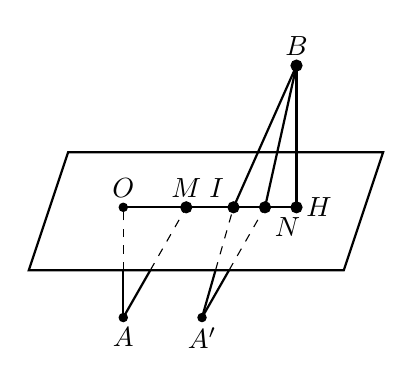
\begin{tikzpicture}
				\coordinate (B) at (3.4,2.6);
				\coordinate (H) at (3.4,0.8);
				\coordinate (N) at (3,0.8);
				\coordinate (I) at (2.6,0.8);
				\coordinate (M) at (2,0.8);
				\coordinate (O) at (1.2,0.8);
				\coordinate (A1) at (1.2,-0.6);
				\coordinate (A2) at (2.2,-0.6);
				\coordinate (T1) at (1.2,0);
				\coordinate (T2) at ({54/35},0);
				\coordinate (T3) at ({83/35},0);
				\coordinate (T4) at ({89/35},0);
				\coordinate (M1) at (0,0);
				\coordinate (M2) at (0.5,1.5);
				\coordinate (M3) at (4.5,1.5);
				\coordinate (M4) at (4,0);
				\draw[thick] (M1) -- (M2) -- (M3) -- (M4) -- cycle;
				\draw[thick] (B) -- (H);
				\draw[thick] (B) -- (N);
				\draw[thick] (B) -- (I);
				\draw[thick] (O) -- (H);
				\draw[thick] (A1) -- (T1);
				\draw[thick] (A1) -- (T2);
				\draw[thick] (A2) -- (T3);
				\draw[thick] (A2) -- (T4);
				\draw[dashed] (T1) -- (O);
				\draw[dashed] (T2) -- (M);
				\draw[dashed] (T3) -- (I);
				\draw[dashed] (T4) -- (N);
				\filldraw (B) circle(2pt) node[above] {$B$};
				\filldraw (H) circle(2pt) node[right] {$H$};
				\filldraw (N) circle(2pt) node[below right] {$N$};
				\filldraw (I) circle(2pt) node[above left] {$I$};
				\filldraw (M) circle(2pt) node[above] {$M$};
				\filldraw (O) circle(1.5pt) node[above] {$O$};
				\filldraw (A1) circle(1.5pt) node[below] {$A$};
				\filldraw (A2) circle(1.5pt) node[below] {$A'$};
			\end{tikzpicture}
		\end{center}
		Từ $\heva{&(S_1) \colon (x-1)^2+(y-1)^2+(z+3)^2=25 (1)\\&(S_2) \colon x^2+y^2+z^2-2x-2y-14=0 (2)}$\\
		Lấy $(1)$ trừ $(2)$, ta được $6z=0$ hay $(P) \colon z=0 \Rightarrow (P) \equiv (Oxy)$.\\
		Dễ thấy $A$, $B$ nằm khác phía đối với $(P)$, hình chiếu của $A$ trên $(P)$ là $O$, hình chiếu của $B$ trên $(P)$ là $H(3;4;0).$\\
		Lấy $A'$ sao cho $\vec{AA'}=\vec{MN}$.\\
		Khi đó $AM+BN=A'N+BN \ge A'B$ và cực trị chỉ xảy ra khi $\vec{MN}$ cùng phương $\vec{OH}$.\\
		Lấy $\vec{MN}=\dfrac{\vec{OH}}{\left| \vec{OH} \right|}=\left(\dfrac{3}{5};\dfrac{4}{5};0\right)$.\\
		Khi đó vì $\vec{AA'}=\vec{MN}$ nên $A'\left(\dfrac{3}{5};\dfrac{4}{5};0\right)$. Do đó $AM+BN=A'N+BN\ge A'B=5$.
	}
\end{ex}

%Câu 17
\begin{ex}%[2H3G1-4]
	Trong KG $Oxyz$ cho mặt cầu $(S)$ có phương trình $x^2+y^2+z^2-4x+2y-2z-3=0$ và điểm $A(5;3;-2)$. Một đường thẳng $d$ thay đổi luôn đi qua $A$ và luôn cắt mặt cầu tại hai điểm phân biệt $M,N$. Tính giá trị nhỏ nhất của biểu thức $S=AM+4AN$.
	\choice
	{$S_{\min} =30$}
	{$S_{\min} =20$}
	{$S_{\min} =\sqrt{34}-3$}
	{\True $S_{\min} =5\sqrt{34}-9$}
	\loigiai{
		Mặt cầu $(S)$ có tâm $I(2;-1;1)$, bán kính $R=3$.\\
		$AI=\sqrt{34}>R \Rightarrow A$ nằm ngoài mặt cầu $(S)$.\\
		\begin{center}
			\begin{tikzpicture}
				\coordinate (M) at ({sqrt(2.3)},{sqrt(1.7)});
				\coordinate (N) at (-{sqrt(3.687286253)},{sqrt(0.3127147469)});
				\coordinate (A) at (-4.5,0);
				\coordinate (I) at (0,0);
				\coordinate (H) at ($(N)!0.5!(M)$);
				\draw[thick] (I) circle (2);
				\draw[thick] (I) -- (A) -- (H) -- cycle;
				\draw[thick] (H) -- (M);
				\filldraw (M) circle(2pt) node[right] {$M$};
				\filldraw (H) circle(2pt) node[above] {$H$};
				\filldraw (N) circle(2pt) node[above left] {$N$};
				\filldraw (A) circle(2pt) node[left] {$A$};
				\filldraw (I) circle(2pt) node[below right] {$I$};
			\end{tikzpicture}
		\end{center}
		Do hai điểm $M,N$ nằm ở vị trí hai đầu một dây cung nên để $S_{\min}$ thì $N$ nằm giữa $A$ và $M$. Gọi $H$ là trung điểm $MN \Rightarrow IH \bot MN, NH=\dfrac{1}{2}MN$.\\ 
		$S=4(AH-NH)+AH+NH=5AH-3NH$\\
		$S=5\sqrt{AI^2-IH^2}-3\sqrt{R^2-IH^2}=5\sqrt{34-x^2}-3\sqrt{9-x^2}, x=IH$\\
		Xét hàm số $f(x)=5\sqrt{34-x^2}-3\sqrt{9-x^2}, (0 \le x < 3)$\\
		$f'(x)=\dfrac{-5x}{\sqrt{34-x^2}}+\dfrac{3x}{\sqrt{9-x^2}}=x \left(\dfrac{-5}{\sqrt{34-x^2}}+\dfrac{3}{\sqrt{9-x^2}}\right)$\\
		Xét $\left(\dfrac{-5}{\sqrt{34-x^2}}+\dfrac{3}{\sqrt{9-x^2}}\right)>0$\\
		$\Leftrightarrow 5\sqrt{9-x^2}<3\sqrt{34-x^2} \Leftrightarrow 225-25x^2<9 \cdot 34-9x^2 \Leftrightarrow 16x^2+81>0$ (luôn đúng).\\
		Suy ra $f'(x) \ge 0, \forall x \in [0;3), f'(x)=0 \Leftrightarrow x=0 \Rightarrow f(x)$ đồng biến trên $[0;3)$\\
		Suy ra $\underset{ [0;3) }{\mathop{\min }}\, f(x)=f(0)=5\sqrt{34}-9$.
	}
\end{ex}

%Câu 18
\begin{ex}%[2H3G1-4]
	Trong KG $Oxyz$ cho đường thẳng $d \colon \dfrac{x-1}{2}=\dfrac{y-2}{3}=\dfrac{z-3}{4}$ và mặt cầu $(S) \colon (x+3)^2+(y+4)^2+(z+5)^2=729$. Cho biết điểm $A(-2;-2;-7)$, điểm $B$ thuộc giao tuyến của mặt cầu $(S)$ và mặt phẳng $(P) \colon 2x+3y+4z-107=0$. Khi điểm $M$ di động trên đường thẳng $d$ giá trị nhỏ nhất của biểu thức $MA+MB$ bằng
	\choice
	{\True $5\sqrt{30}$}
	{$27$}
	{$5\sqrt{29}$}
	{$\sqrt{742}$}
	\loigiai{
		\begin{center}
			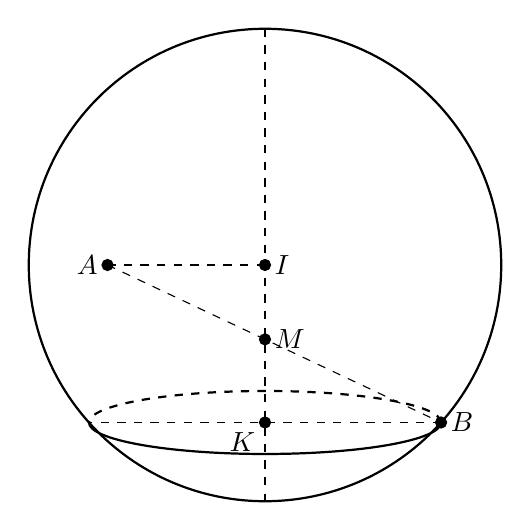
\begin{tikzpicture}
				\coordinate (P1) at (0,3);
				\coordinate (I) at (0,0);
				\coordinate (A) at (-2,0);
				\coordinate (M) at (0,-0.9442719);
				\coordinate (B) at (2.236068,-2);
				\coordinate (K) at (0,-2);
				\coordinate (P2) at (-2.236068,-2);
				\coordinate (P3) at (0,-3);
				\draw[thick] (I) circle(3);
				\draw[dashed] (P1) -- (P3);
				\draw[dashed] (I) -- (A);
				\draw[dashed] (A) -- (B);
				\draw[dashed] (B) -- (P2);
				\def\a{2.2360678}
				\def\b{0.4}
				\draw[dashed, thick] (2.236068,-2) arc[start angle=0, end angle=180, x radius=\a, y radius=\b];
				\draw[thick] (-2.236068,-2) arc[start angle=180, end angle=360, x radius=\a, y radius=\b];
				\filldraw (I) circle(2pt) node[right] {$I$};
				\filldraw (A) circle(2pt) node[left] {$A$};
				\filldraw (M) circle(2pt) node[right] {$M$};
				\filldraw (B) circle(2pt) node[right] {$B$};
				\filldraw (K) circle(2pt) node[below left] {$K$};
			\end{tikzpicture}
		\end{center}
		Mặt cầu $(S)$ có tâm $I(-3;-4;-5)$ và bán kính $R=27$.\\
		Đường thẳng $d$ có 1 véc-tơ chỉ phương là $\vec{u}=(2;3;4)\Rightarrow d\bot(P)$.\\
		Gọi $K$ là giao điểm của mặt phẳng $(P)$ và đường thẳng $d$. Vì $I\in d$ nên $K$ là tâm của đường tròn giao tuyến và $KB\bot d$.\\
		Ta có $\vec{IA}=(1;2;-2)\Rightarrow IA=3$ và $\vec{IA}.\vec{u}=0\Rightarrow IA\bot d$.\\
		Ta tính được $IK=\text{d(I,(P))}=\dfrac{\left| 2 \cdot (-3)+3 \cdot (-4)+4(-5)-107 \right|}{\sqrt{2^2+3^2+4^2}}=5\sqrt{29}$\\ Và $KB=\sqrt{R^2-IK^2}=2$.\\
		Do $M$ di động trên đường thẳng $d$ (trục của đường tròn giao tuyến) và $B$ thuộc đường tròn giao tuyến nên biểu thức $MA+MB$ nhỏ nhất khi và chỉ khi $M=AB\cap d$.\\
		Khi đó, ta có $\dfrac{MI}{MK}=\dfrac{IA}{KB}=\dfrac{3}{2}$ và $MI+MK=IK=5\sqrt{29}$.\\
		Suy ra $MI=3\sqrt{29}$, $MK=2\sqrt{29}$.\\
		Ta có $AM=\sqrt{IA^2+MI^2}=3\sqrt{30}\Rightarrow BM=\dfrac{2}{3}AM=2\sqrt{30}$.\\
		Vậy giá trị nhỏ nhất của $MA+MB$ là $AM+BM=3\sqrt{30}+2\sqrt{30}=5\sqrt{30}$.\\
		Cách 2:
		Ta có $(S)$ có tâm $I(-3;-4;-5)$, bán kính $R=27$.\\
		Dễ thấy $d$ đi qua $I(-3;-4;-5)$và vuông góc với $(P)$.\\
		$(P)$ cắt $(S)$ theo đường tròn có bán kính $r=2$.
		$M\in d\Leftrightarrow M(1+2t;2+3t;3+4t)$.\\
		Ta có $T=MA+MB=MA+\sqrt{MH^2+r^2}$.\\
		Lại có $MH=d(M;(P))=\dfrac{\left| 29t-87 \right|}{\sqrt{29}}=\left| \sqrt{29}t-3\sqrt{29}\right|$.\\
		Suy ra\\ $T=\sqrt{29t^2+116t+125}+\sqrt{29(t-3)^2+4}$\\
		$T=\sqrt{29}\sqrt{(t+2)^2+\dfrac{9}{29}}+\sqrt{29}\sqrt{(t-3)^2+\dfrac{4}{29}}$.\\
		Xét $\vec{u}=\left(t+2;\dfrac{3}{\sqrt{29}}\right)$, $\vec{v}=\left(3-t;\dfrac{2}{\sqrt{29}}\right)\Rightarrow \vec{u}+\vec{v}=\left(5;\dfrac{5}{\sqrt{29}}\right)$.\\
		Do đó $T=\sqrt{29}(\left| \vec{u} \right|+\left| \vec{v} \right|) \ge \sqrt{29}\left| \vec{u}+\vec{v} \right|=5\sqrt{50}$.
	}
\end{ex}

%Câu 19
\begin{ex}%[2H3G1-4]
	Trong không gian với hệ trục tọa độ $Oxyz$, cho hai mặt cầu $(S_1) \colon x^2+y^2+z^2=1$, $(S_2) \colon x^2+(y-4)^2+z^2=4$ và các điểm $A(4;0;0)$, $B\left(\dfrac{1}{4};0;0\right)$, $C(1;4;0)$, $D(4;4;0)$. Gọi $M$ là điểm thay đổi trên $(S_1)$, $N$ là điểm thay đổi trên $(S_2)$. Giá trị nhỏ nhất của biểu thức $Q=MA+2ND+4MN+4BC$ là
	\choice
	{\True $2\sqrt{265}$}
	{$\sqrt{265}$}
	{$3\sqrt{265}$}
	{$4\sqrt{265}$}
	\loigiai{
		\begin{center}
			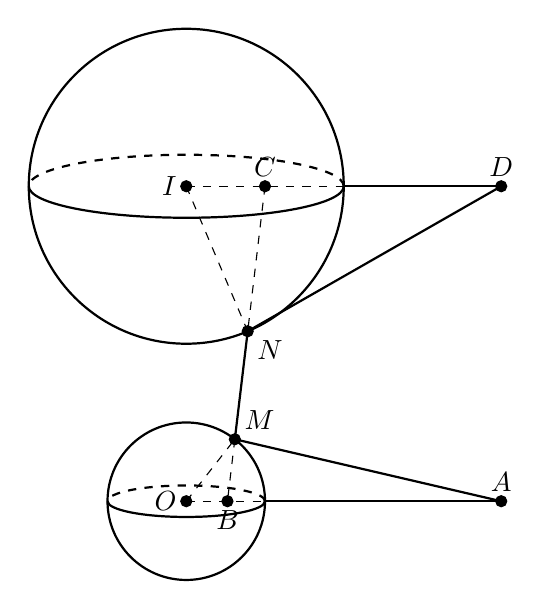
\begin{tikzpicture}
				\coordinate (I) at (0,4);
				\coordinate (C) at (1,4);
				\coordinate (D) at (4,4);
				\coordinate (N) at (0.78041,2.158544);
				\coordinate (M) at (0.616865765,0.7870683);
				\coordinate (O) at (0,0);
				\coordinate (B) at (0.523,0);
				\coordinate (A) at (4,0);
				\coordinate (P1) at (2,4);
				\coordinate (P2) at (1,0);
				\draw [thick] (O) circle(1);
				\draw [thick] (I) circle(2);
				\draw [dashed] (I) -- (P1);
				\draw [dashed] (I) -- (N);
				\draw [dashed] (C) -- (N);
				\draw [dashed] (O) -- (M);
				\draw [dashed] (O) -- (P2);
				\draw [dashed] (M) -- (B);
				\draw [thick] (P1) -- (D);
				\draw [thick] (N) -- (D);
				\draw [thick] (N) -- (M);
				\draw [thick] (M) -- (A);
				\draw [thick] (P2) -- (A);
				\draw[dashed, thick] (2,4) arc[start angle=0, end angle=180, x radius=2, y radius=0.4];
				\draw[thick] (-2,4) arc[start angle=180, end angle=360, x radius=2, y radius=0.4];
				\draw[dashed, thick] (1,0) arc[start angle=0, end angle=180, x radius=1, y radius=0.2];
				\draw[thick] (-1,0) arc[start angle=180, end angle=360, x radius=1, y radius=0.2];
				\filldraw (I) circle(2pt) node[left] {$I$};
				\filldraw (C) circle(2pt) node[above] {$C$};
				\filldraw (D) circle(2pt) node[above] {$D$};
				\filldraw (N) circle(2pt) node[below right] {$N$};
				\filldraw (M) circle(2pt) node[above right] {$M$};
				\filldraw (O) circle(2pt) node[left] {$O$};
				\filldraw (B) circle(2pt) node[below] {$B$};
				\filldraw (A) circle(2pt) node[above] {$A$};
			\end{tikzpicture}
		\end{center}
		$(S_1): x^2 + y^2 + z^2 = 1$ nên $(S_1)$ có tâm $O(0;0;0)$ và bán kính $R_1 = 1$.\\
		$(S_2): x^2 + (y-4)^2 + z^2 = 4$ nên $(S_2)$ có tâm $I(0;4;0)$ và bán kính $R_2 = 2$.\\
		Vậy các điểm $A(4;0;0)$, $B\left(\dfrac{1}{4};0;0\right)$, $C(1;4;0)$, $D(4;4;0)$, $O(0;0;0)$ và $I(0;4;0)$ cùng thuộc $(Oxy)$.\\
		Nhận thấy $OB \cdot OA = OM^2$ suy ra $OM$ là tiếp tuyến của đường tròn ngoại tiếp tam giác $MAB$.\\
		Do đó $\Delta MOB$ đồng dạng $\Delta AOM$.\\
		$\Rightarrow \dfrac{MA}{MB} = \dfrac{OA}{OM} = 4 \Rightarrow MA = 4MB$.\\
		Hoàn toàn tương tự $\dfrac{ND}{NC} = \dfrac{DI}{NI} = 2 \Rightarrow ND = 2NC$.\\
		Xét:\\
		$Q = MA + 2ND + 4MN + 4BC$\\
		$Q = 4(MB + NC + MN) + 4BC \ge 4BC + 4BC = 8BC = 2\sqrt{265}$.
	}
\end{ex}